\begin{figure}[h] 
\centering 
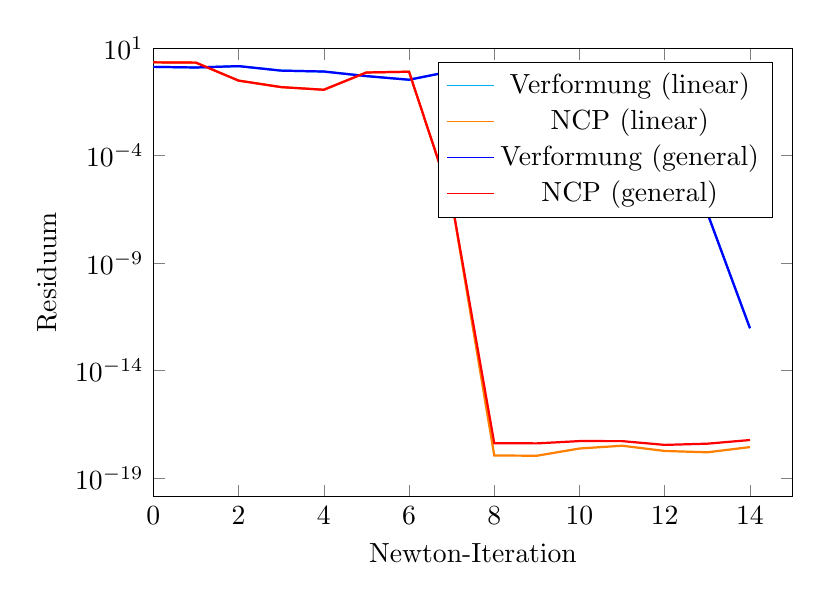
\begin{tikzpicture}[every plot/.append style={thick}] 
\begin{axis}[ 
label style={font=\normalsize}, 
xlabel={Newton-Iteration}, 
ylabel={Residuum}, 
xmin=0, xmax=15, 
ymode=log, 
ymin=0, ymax=10, 
width=0.8\textwidth, 
height=0.6\textwidth, 
legend pos=north east, 
legend style={cells={align=left}}, 
grid style=dashed, 
] 
\addplot[ 
color=cyan, 
] 
coordinates { 
(0, 1.35e+00)(1, 1.26e+00)(2, 1.46e+00)(3, 9.01e-01)(4, 8.18e-01)(5, 5.01e-01)(6, 3.39e-01)(7, 8.44e-01)(8, 2.07e-01)(9, 5.38e-02)(10, 9.93e-03)(11, 3.04e-03)(12, 1.58e-04)(13, 2.12e-07)(14, 9.25e-13)}; 
\addlegendentry{Verformung (linear)} 
\addplot[ 
color=orange, 
] 
coordinates { 
(0, 2.19e+00)(1, 2.12e+00)(2, 3.09e-01)(3, 1.54e-01)(4, 1.16e-01)(5, 7.39e-01)(6, 8.00e-01)(7, 8.12e-07)(8, 1.11e-18)(9, 1.08e-18)(10, 2.34e-18)(11, 3.16e-18)(12, 1.80e-18)(13, 1.56e-18)(14, 2.73e-18)}; 
\addlegendentry{NCP (linear)} 
\addplot[ 
color=blue, 
] 
coordinates { 
(0, 1.35e+00)(1, 1.26e+00)(2, 1.46e+00)(3, 9.01e-01)(4, 8.18e-01)(5, 5.01e-01)(6, 3.39e-01)(7, 8.44e-01)(8, 2.07e-01)(9, 5.38e-02)(10, 9.93e-03)(11, 3.04e-03)(12, 1.58e-04)(13, 2.12e-07)(14, 9.25e-13)}; 
\addlegendentry{Verformung (general)} 
\addplot[ 
color=red, 
] 
coordinates { 
(0, 2.19e+00)(1, 2.12e+00)(2, 3.09e-01)(3, 1.54e-01)(4, 1.16e-01)(5, 7.39e-01)(6, 8.00e-01)(7, 8.12e-07)(8, 4.16e-18)(9, 4.06e-18)(10, 5.19e-18)(11, 5.17e-18)(12, 3.45e-18)(13, 3.93e-18)(14, 5.81e-18)}; 
\addlegendentry{NCP (general)} 
\end{axis} 
\end{tikzpicture} 
\caption{Residuen des Stoffgesetzes 'St.Venant' mit Hinderniss 'Spitze' und 2178 Freiheitsgraden für die Verschiebung.} 
\label{fiq:St.Venant_Spitze_level4} 
\end{figure} 
